% Created 2017-10-11 Wed 11:15
\documentclass[presentation]{beamer}
\usepackage[utf8]{inputenc}
\usepackage[T1]{fontenc}
\usepackage{fixltx2e}
\usepackage{graphicx}
\usepackage{longtable}
\usepackage{float}
\usepackage{wrapfig}
\usepackage{rotating}
\usepackage[normalem]{ulem}
\usepackage{amsmath}
\usepackage{textcomp}
\usepackage{marvosym}
\usepackage{wasysym}
\usepackage{amssymb}
\usepackage{hyperref}
\tolerance=1000
\usepackage{graphicx}
\usetheme{simple}
\usecolortheme{}
\usefonttheme{serif}
\useinnertheme{}
\useoutertheme{}
\author{Talon Chandler}
\date{October 11, 2017}
\title{Progress Report On Orientation Determination With Maximum Likelihood Methods}
\hypersetup{
  pdfkeywords={},
  pdfsubject={},
  pdfcreator={Emacs 25.3.1 (Org mode 8.2.10)}}
\begin{document}

\maketitle
\begin{frame}[label=sec-1]{Microscope Geometry}
\begin{center}
  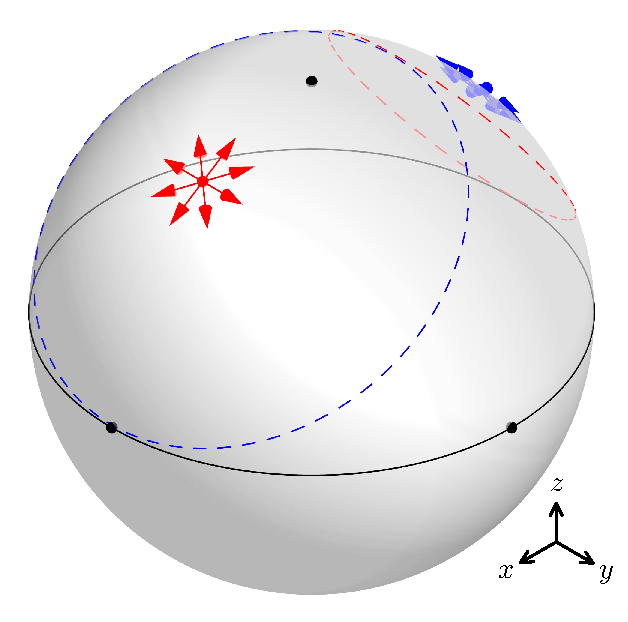
\includegraphics[width=0.5\textwidth, interpolate=true]{figs/geometry.pdf}\\
  1.1 and 0.71 NA\\
  8 Poisson-distributed intensity measurements\\
  Goal: Estimate the orientation of the dipole.
\end{center}
\end{frame}
\begin{frame}[label=sec-2]{Fisher Scoring Algorithm}
\begin{center}
\begin{align*}
  \vec{\theta} = \{\Theta, \Phi\} &\rightarrow \text{Parameters}\\
  \vec{X}  &\rightarrow \text{Data (8 intensity measurements)}\\
  \textbf{F}(\vec{\theta}) &\rightarrow \text{Fisher information matrix}\\
  \vec{V}(\vec{\theta}, \vec{X}) = \frac{\partial}{\partial \vec{\theta}} \log L(\vec{\theta}, \vec{X}) &\rightarrow \text{Score}
\end{align*}
\begin{align*}
  \vec{\theta}_{i+1} = \vec{\theta}_{i} + \textbf{F}^{-1}(\vec{\theta})\vec{V}(\vec{\theta}, \vec{X})
\end{align*}
\end{center}
\end{frame}
\begin{frame}[label=sec-3]{Fisher Scoring Run 1}
\begin{center}
True orientation: $\Theta = \pi/2, \Phi = \pi/4$\\
Starting orientation: $\Theta = \pi/3, \Phi = \pi/3$
  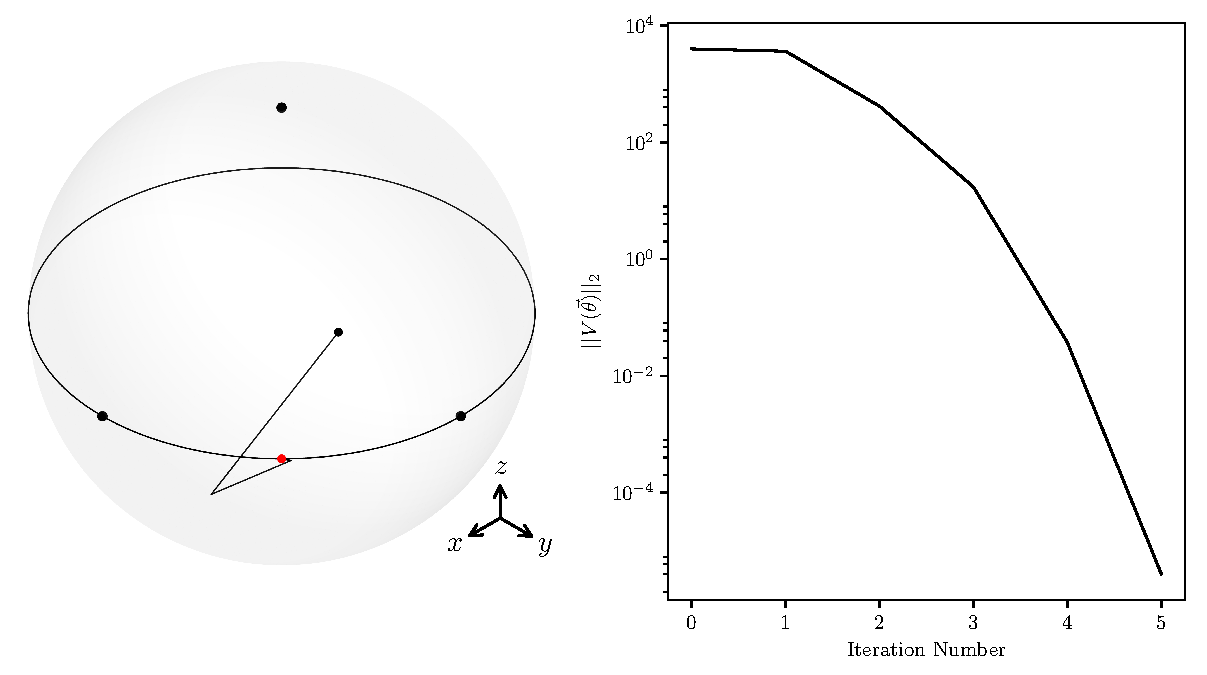
\includegraphics[width=1.0\textwidth, interpolate=true]{figs/recon-history1.pdf}
\end{center}
\end{frame}
\begin{frame}[label=sec-4]{Fisher Scoring Run 2}
\begin{center}
True orientation: $\Theta = \pi/2, \Phi = \pi/4$\\
Starting orientation: $\Theta = \pi/3, \Phi = \pi/2$
  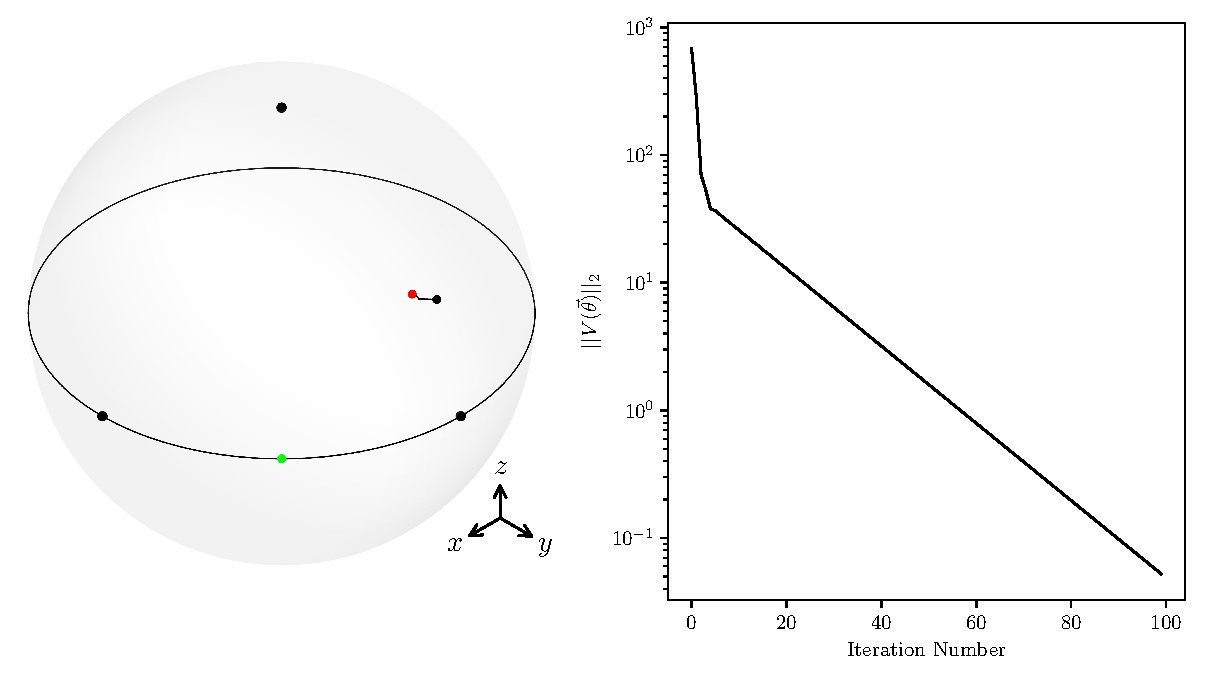
\includegraphics[width=1.0\textwidth, interpolate=true]{figs/recon-history2.pdf}
\end{center}
\end{frame}
\begin{frame}[label=sec-5]{Fisher Scoring Run 3}
\begin{center}
True orientation: $\Theta = \pi/2, \Phi = \pi/4$\\
Starting orientation: $\Theta = 0, \Phi = 0$
  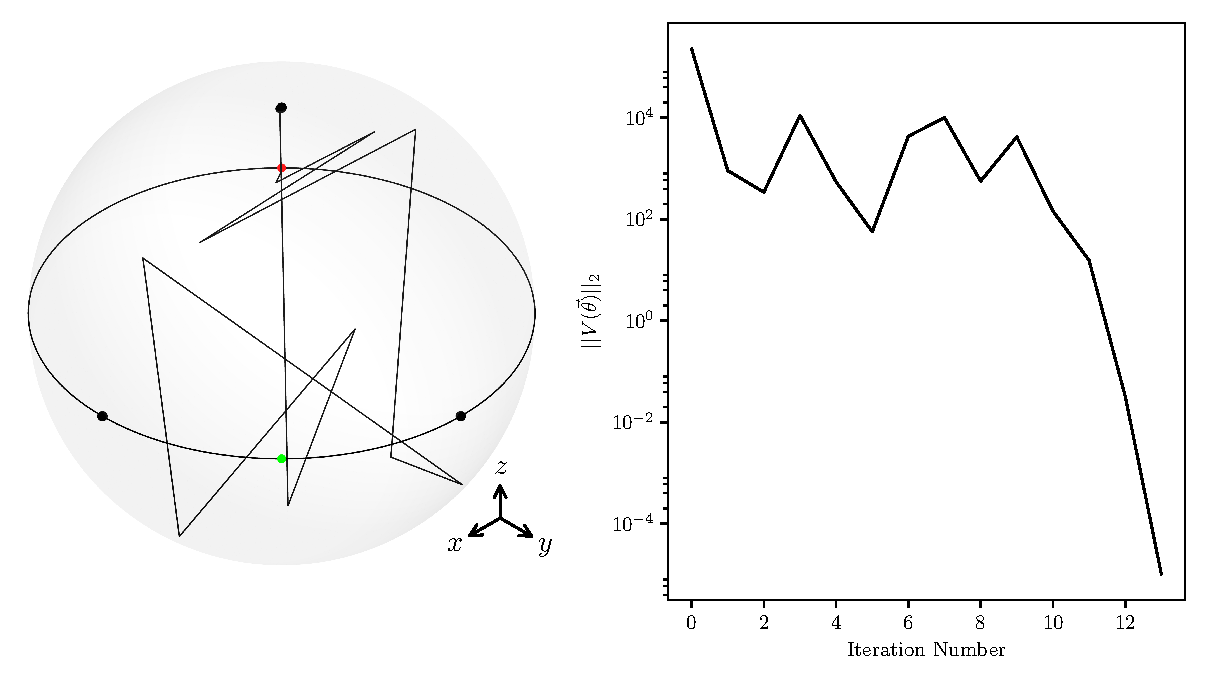
\includegraphics[width=1.0\textwidth, interpolate=true]{figs/recon-history3.pdf}
\end{center}
\end{frame}
\begin{frame}[label=sec-6]{Log-likelihood as a function of the estimate orientation}
  \begin{center}
  True orientation: $\Theta = \pi/2, \Phi = \pi/4$\\
    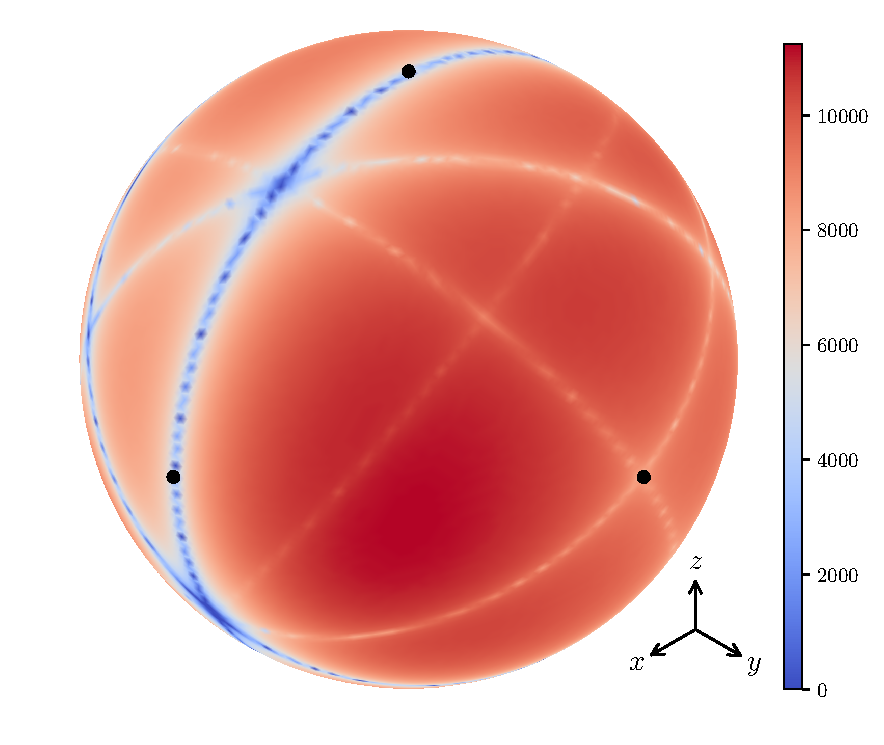
\includegraphics[width=0.55\textwidth, interpolate=true]{figs/likelihood.pdf}\\
Gradient descent isn't going to cut it.\\
I need to be careful with derivatives on curved spaces. 
  \end{center}
\end{frame}


\begin{frame}[label=sec-7]{Log-likelihood as a function of the estimate orientation}
\begin{center}
True orientation: $\Theta = 0, \Phi = 0$\\
  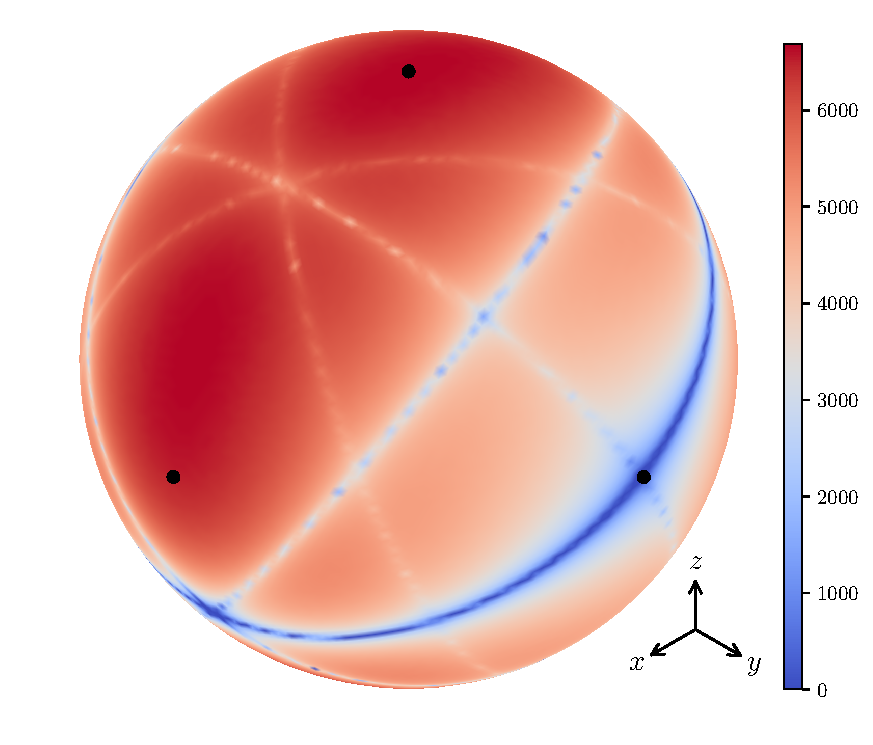
\includegraphics[width=0.55\textwidth, interpolate=true]{figs/likelihood2.pdf}\\
\end{center}
\end{frame}

\begin{frame}[label=sec-8]{Brute Force Optimization}
Choose number of points (100). \\
Plot error in degrees (great circle arc) between truth and estimate as a function of truth. \\
\begin{center}
  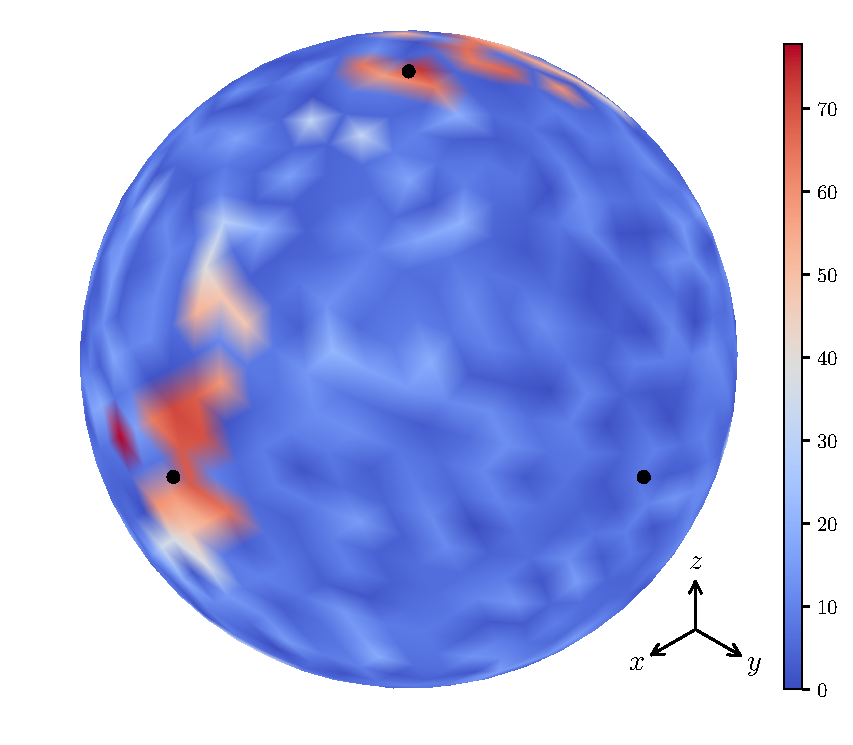
\includegraphics[width=0.55\textwidth, interpolate=true]{figs/angle-error-brute.pdf}\\
\end{center}
\end{frame}
\begin{frame}[label=sec-9]{Particle Swarm Optimization}
Choose starting number of points (25). \\
    Choose max number of function evaluations (100). \\
    Plot error in degrees (great circle arc) between truth and estimate as a function of truth. \\
\begin{center}
  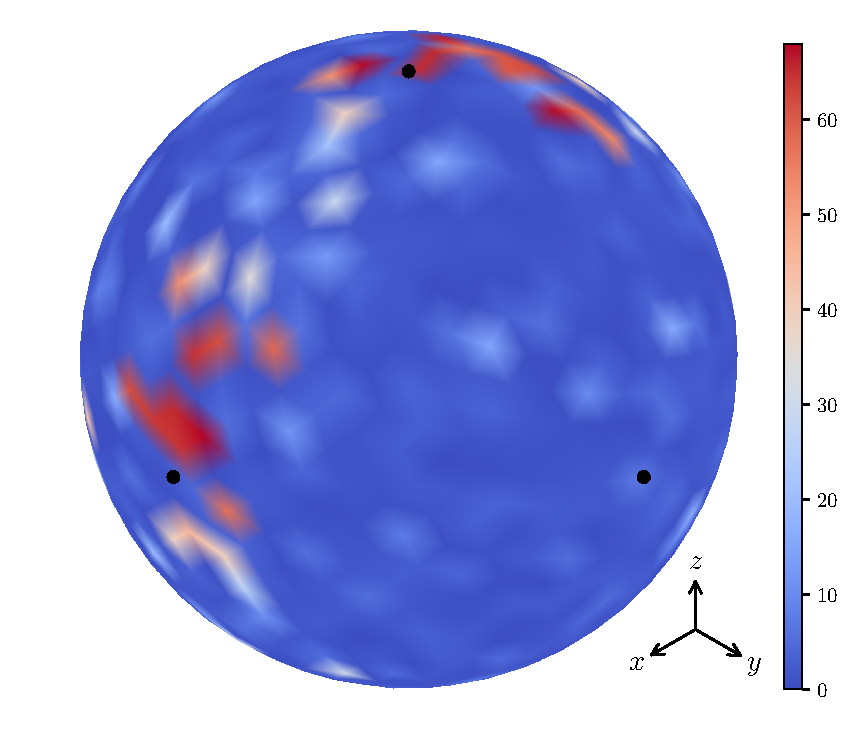
\includegraphics[width=0.55\textwidth, interpolate=true]{figs/angle-error.pdf}\\
\end{center}
\end{frame}
% Emacs 25.3.1 (Org mode 8.2.10)
\end{document}